\section{Probabilistic catalogs based on the 3FGL and 4FGL catalogs}


Having optimized our algorithms, we decided to test them on 3FGL data which was initially unassociated but then became associated in 4FGL. Furthermore, we tested the algorithms on 4FGL associated data, and also predicted for unassociated data.
\subsection{Prediction for unassociated sources in 3FGL and comparison with 4FGL}
\lb{sec:3FGLprediction1}


In this section we use the algorithms from the previous section to predict classes for the unassociated sources in the 3FGL. 
We have selected the following four algorithms: RF with 50 trees and max depth of 6, BDT with 100 trees and max depth of 2, NN with 10 neurons, Adam solver, and 300 epochs, and LR with LBFGS solver and 200 iterations. We use unweighted data to train all of the algorithms.

The details of the selected algorithms are summarized in Table \ref{tab:selected_algs}.
``Average testing accuracy'' is computed by taking 1000 times 70\% - 30\% split into training and testing samples and averaging over the 
accuracies computed for the testing samples.
In addition, we look at sources, which are unassociated in 3FGL but have either pulsar or AGN association in 4FGL: there are 278 such sources.
The accuracy of our prediction for the four selected algorithms, taking the 4FGL classes as the true values, is reported in the column ``Accuracy from Comparison with 4FGL''.
The correct classifications and misclassifications for the 278 sources with associations in 4FGL are also presented in Figure \ref{fig:3FGL_vs_4FGL_classes}.
The class at the beginning of the label names corresponds to the association in the 4FGL, while the second half of the labels corresponds to classification of unassociated sources in 3FGL, for example, ``PSRs classified only as PSRs'' shows sources which have PSR association in 4FGL and all four algorithms classified the corresponding unassociated sources in 3FGL as PSRs, while ``PSRs classified as either PSRs or AGNs'' labels sources with PSR associations in 4FGL but the corresponding unassociated sources in 3FGL have both PSR and AGN classifications by different ML algorithms.
The unassociated sources are classified as PSRs or AGNs if the corresponding probability is larger than 0.5.
We notice that misclassified or partially misclassified sources in Figure \ref{fig:3FGL_vs_4FGL_classes} typically happen on the boundary between the two classes or even inside the opposite class.
Many of these sources also have flags in the 3FGL catalog, such as a potential problem with the background diffuse emission model in the location of the source, which can lead to a poor reconstruction of the source spectrum and, as a result, misclassification of the source.

%Here we discuss the results of our probabilistic classification on the unassociated data. The 242 sources for whom FGL counterparts existed were plotted in figure 10. This figure shows all AGNs and PSRs, including those which were correctly or incorrectly identified by all the 4 algorithms (given by keyword only) and those which are a mix of correct and incorrect classification by at least one of the 4 algorithms (given by keywords either/or). 



\begin{table}[!h]

\resizebox{0.45\textwidth}{!}{
    \tiny
 %  \centering
    \renewcommand{\tabcolsep}{0.3mm}
\renewcommand{\arraystretch}{1.5}

    \begin{tabular}{|c|c|c|c|}
    \hline
    Algorithm&Parameters & Average  & Accuracy from \\
    & & Testing Accuracy & Comparison with 4FGL\\
    \hline
    RF& 50 trees, max depth 6  &97.42& 96.1  \\
    \hline %\midrule   -> aakash do you mean this?
    BDT & 100 trees, max depth 2    &   97.80&95.34 \\
%    \hline %\midrule   -> aakash do you mean this?
%    BDT & 200 trees, max depth 2    &   95.8  \\
    \hline
    NN & 300, 10 Neurons, Adam & 97.40& 94.55\\
    \hline
    LR & LBFGS solver, 200 iterations & 97.60& 93.48 \\
    \hline
     
    \end{tabular}}
    \vspace{0.2cm}
    \caption{Accuracy of the 4 selected algorithms on 3FGL unassociated data.}
    \label{tab:selected_algs}
\end{table}

\begin{figure*}[h]
\centering
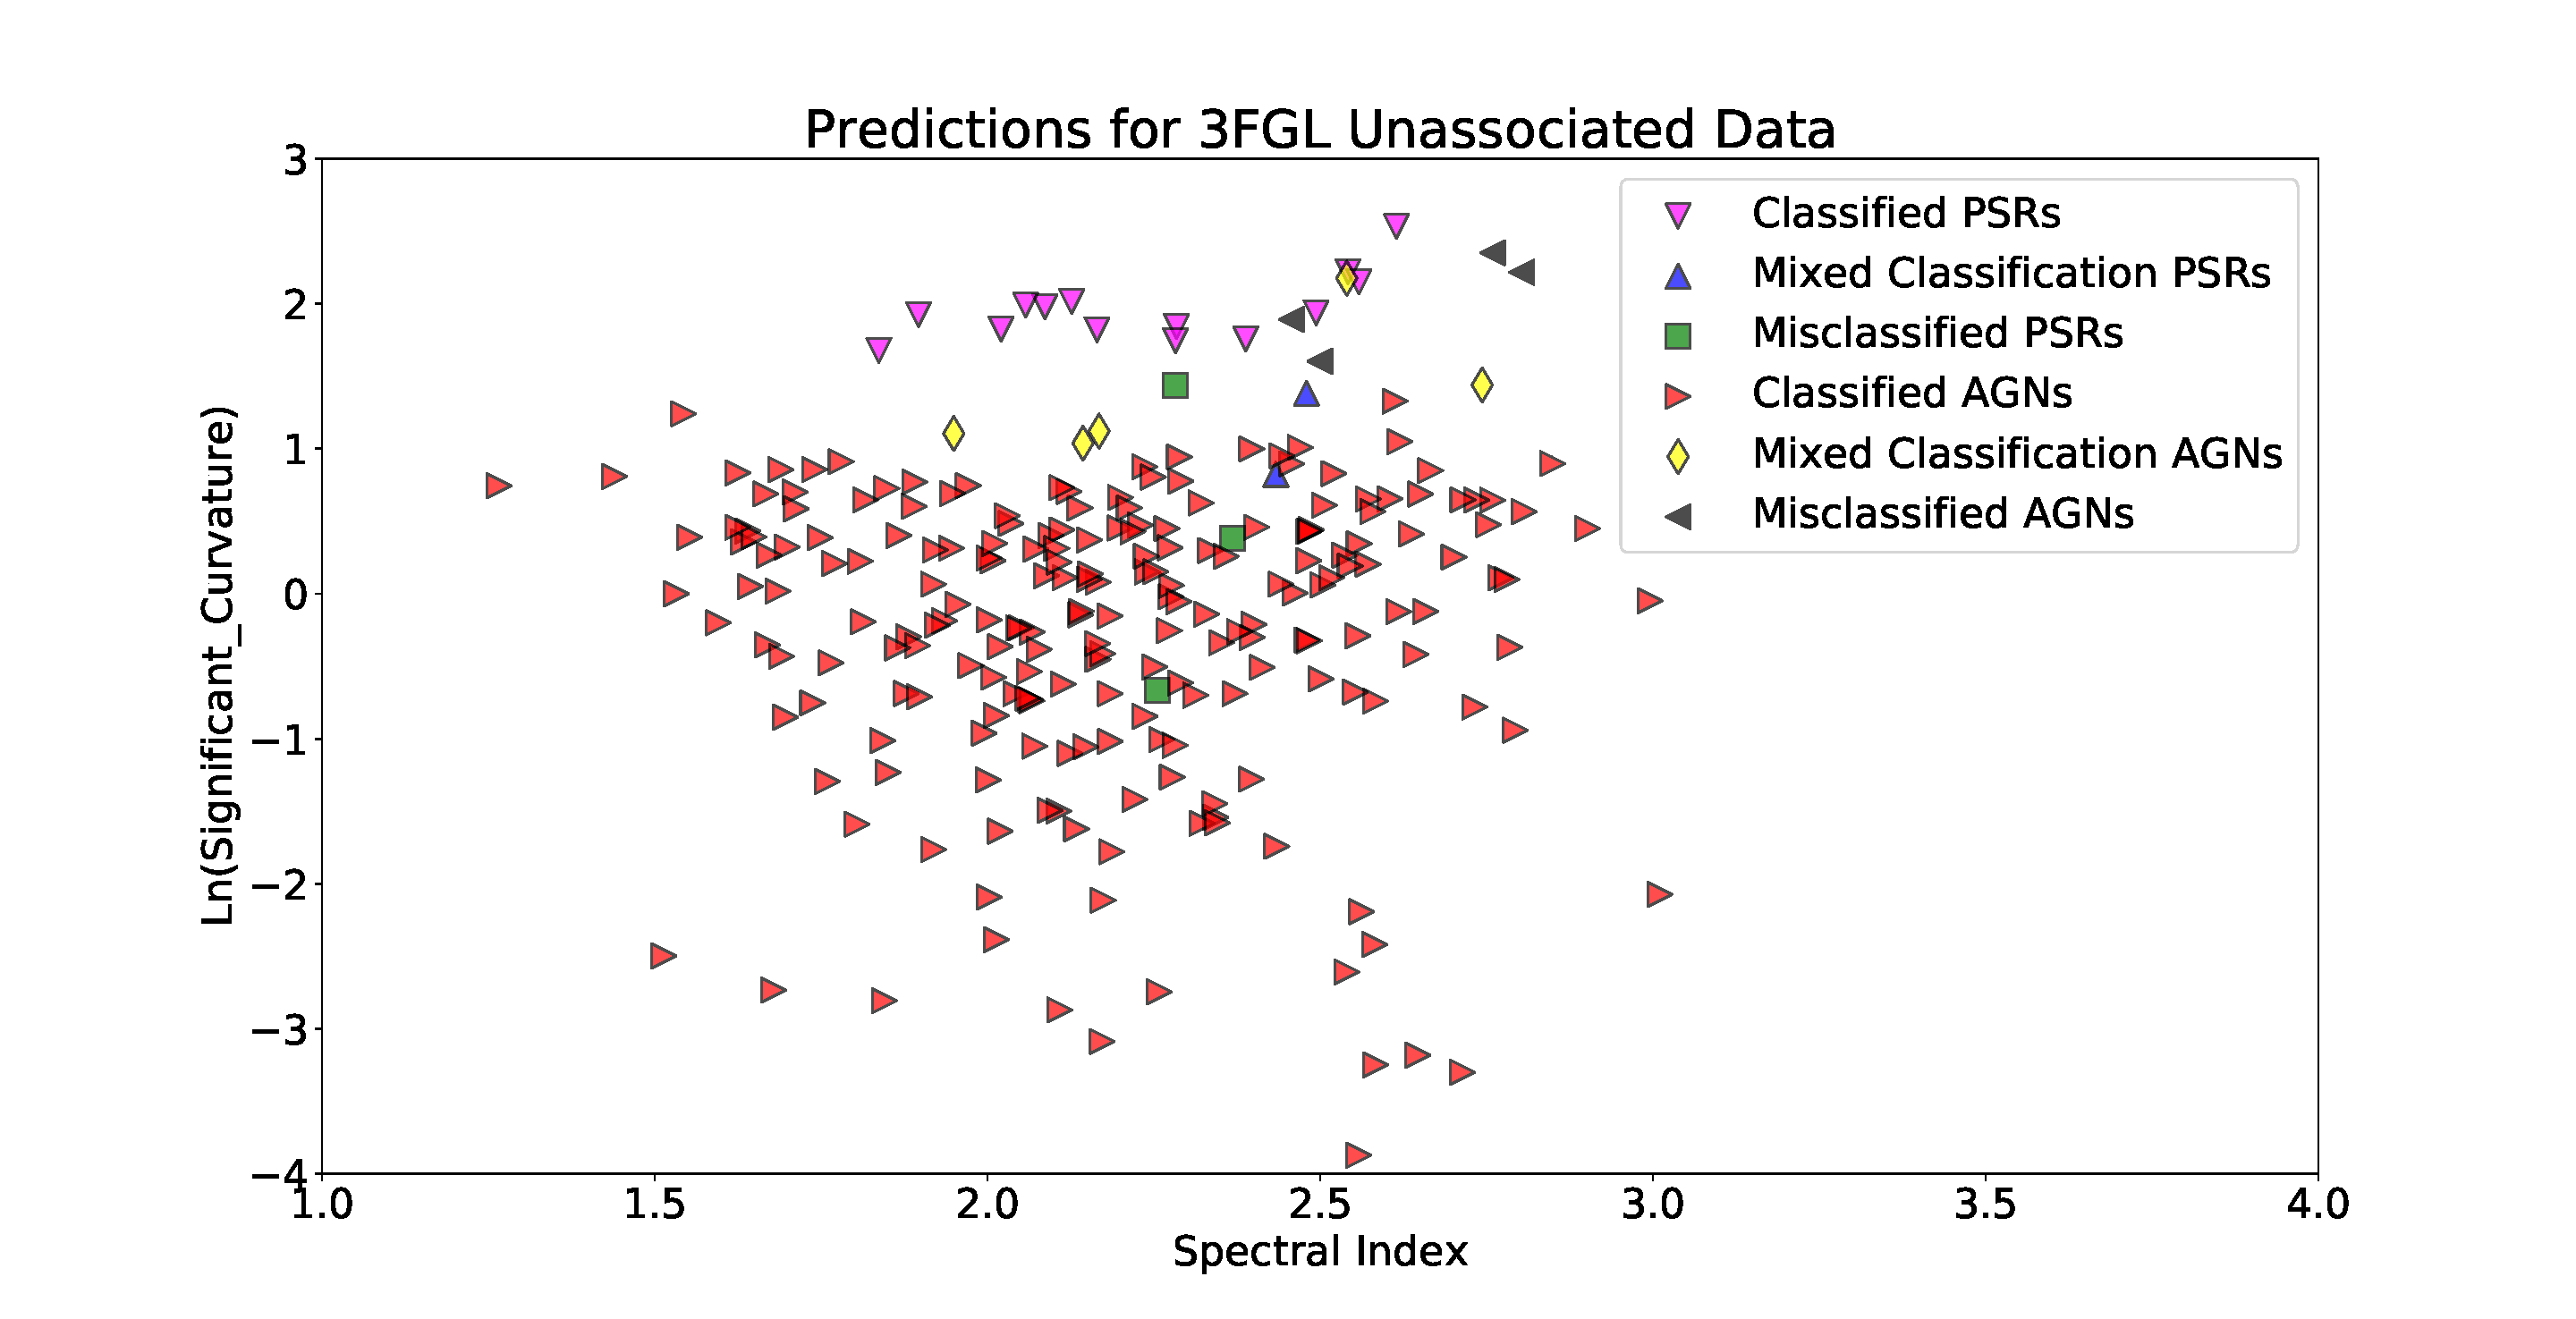
\includegraphics[width=0.8\textwidth]{plots/plot_final.pdf}
%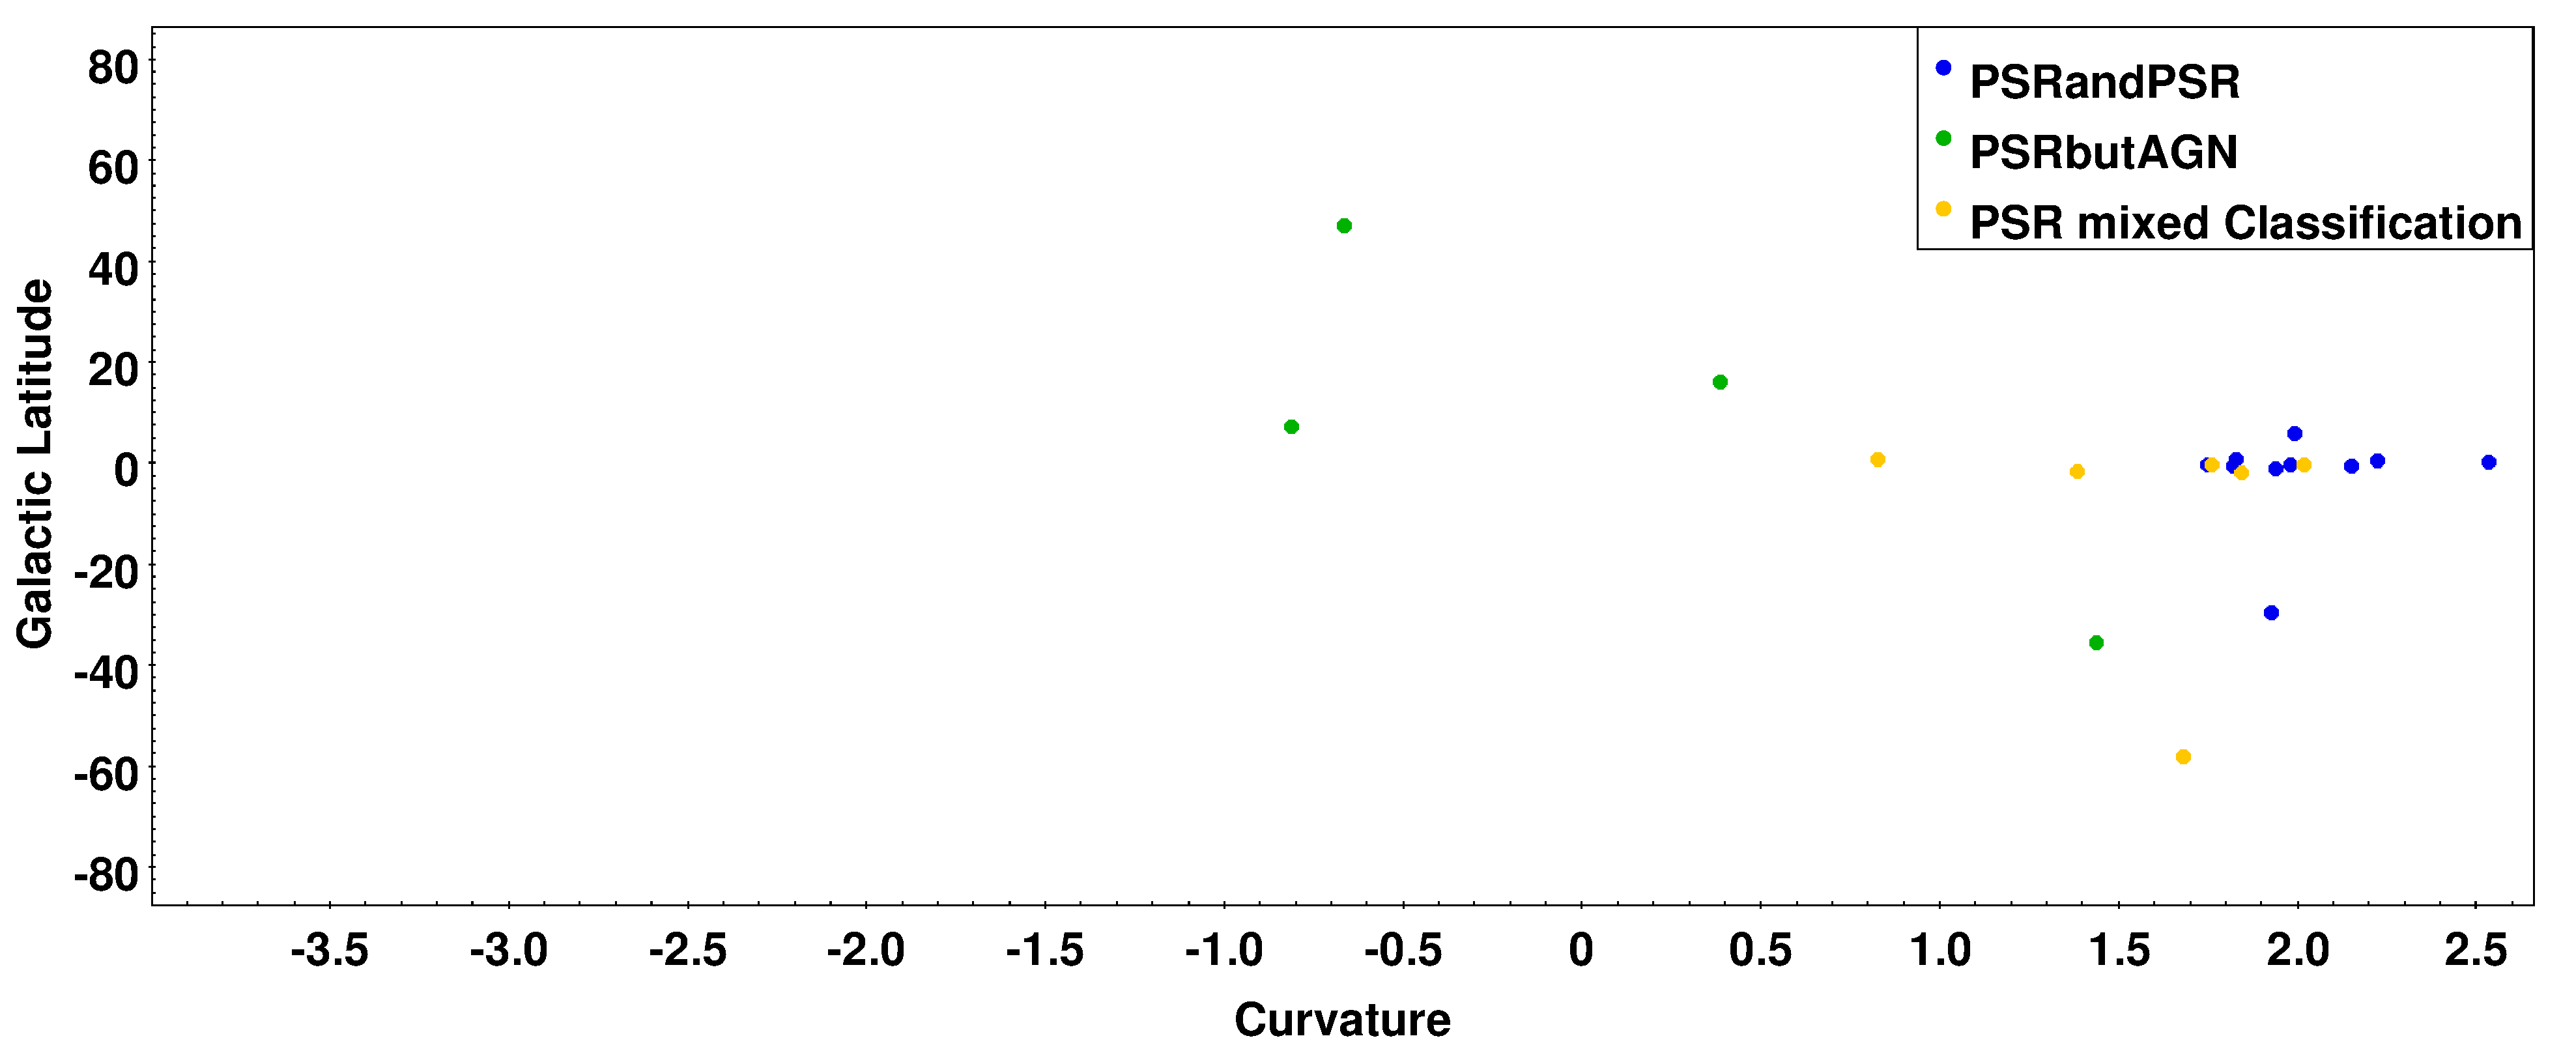
\includegraphics[width=\twopicsp\textwidth]{plots/PSR3.pdf}
\caption{Comparison of class prediction for unassociated 3FGL sources with classes in 4FGL. }
%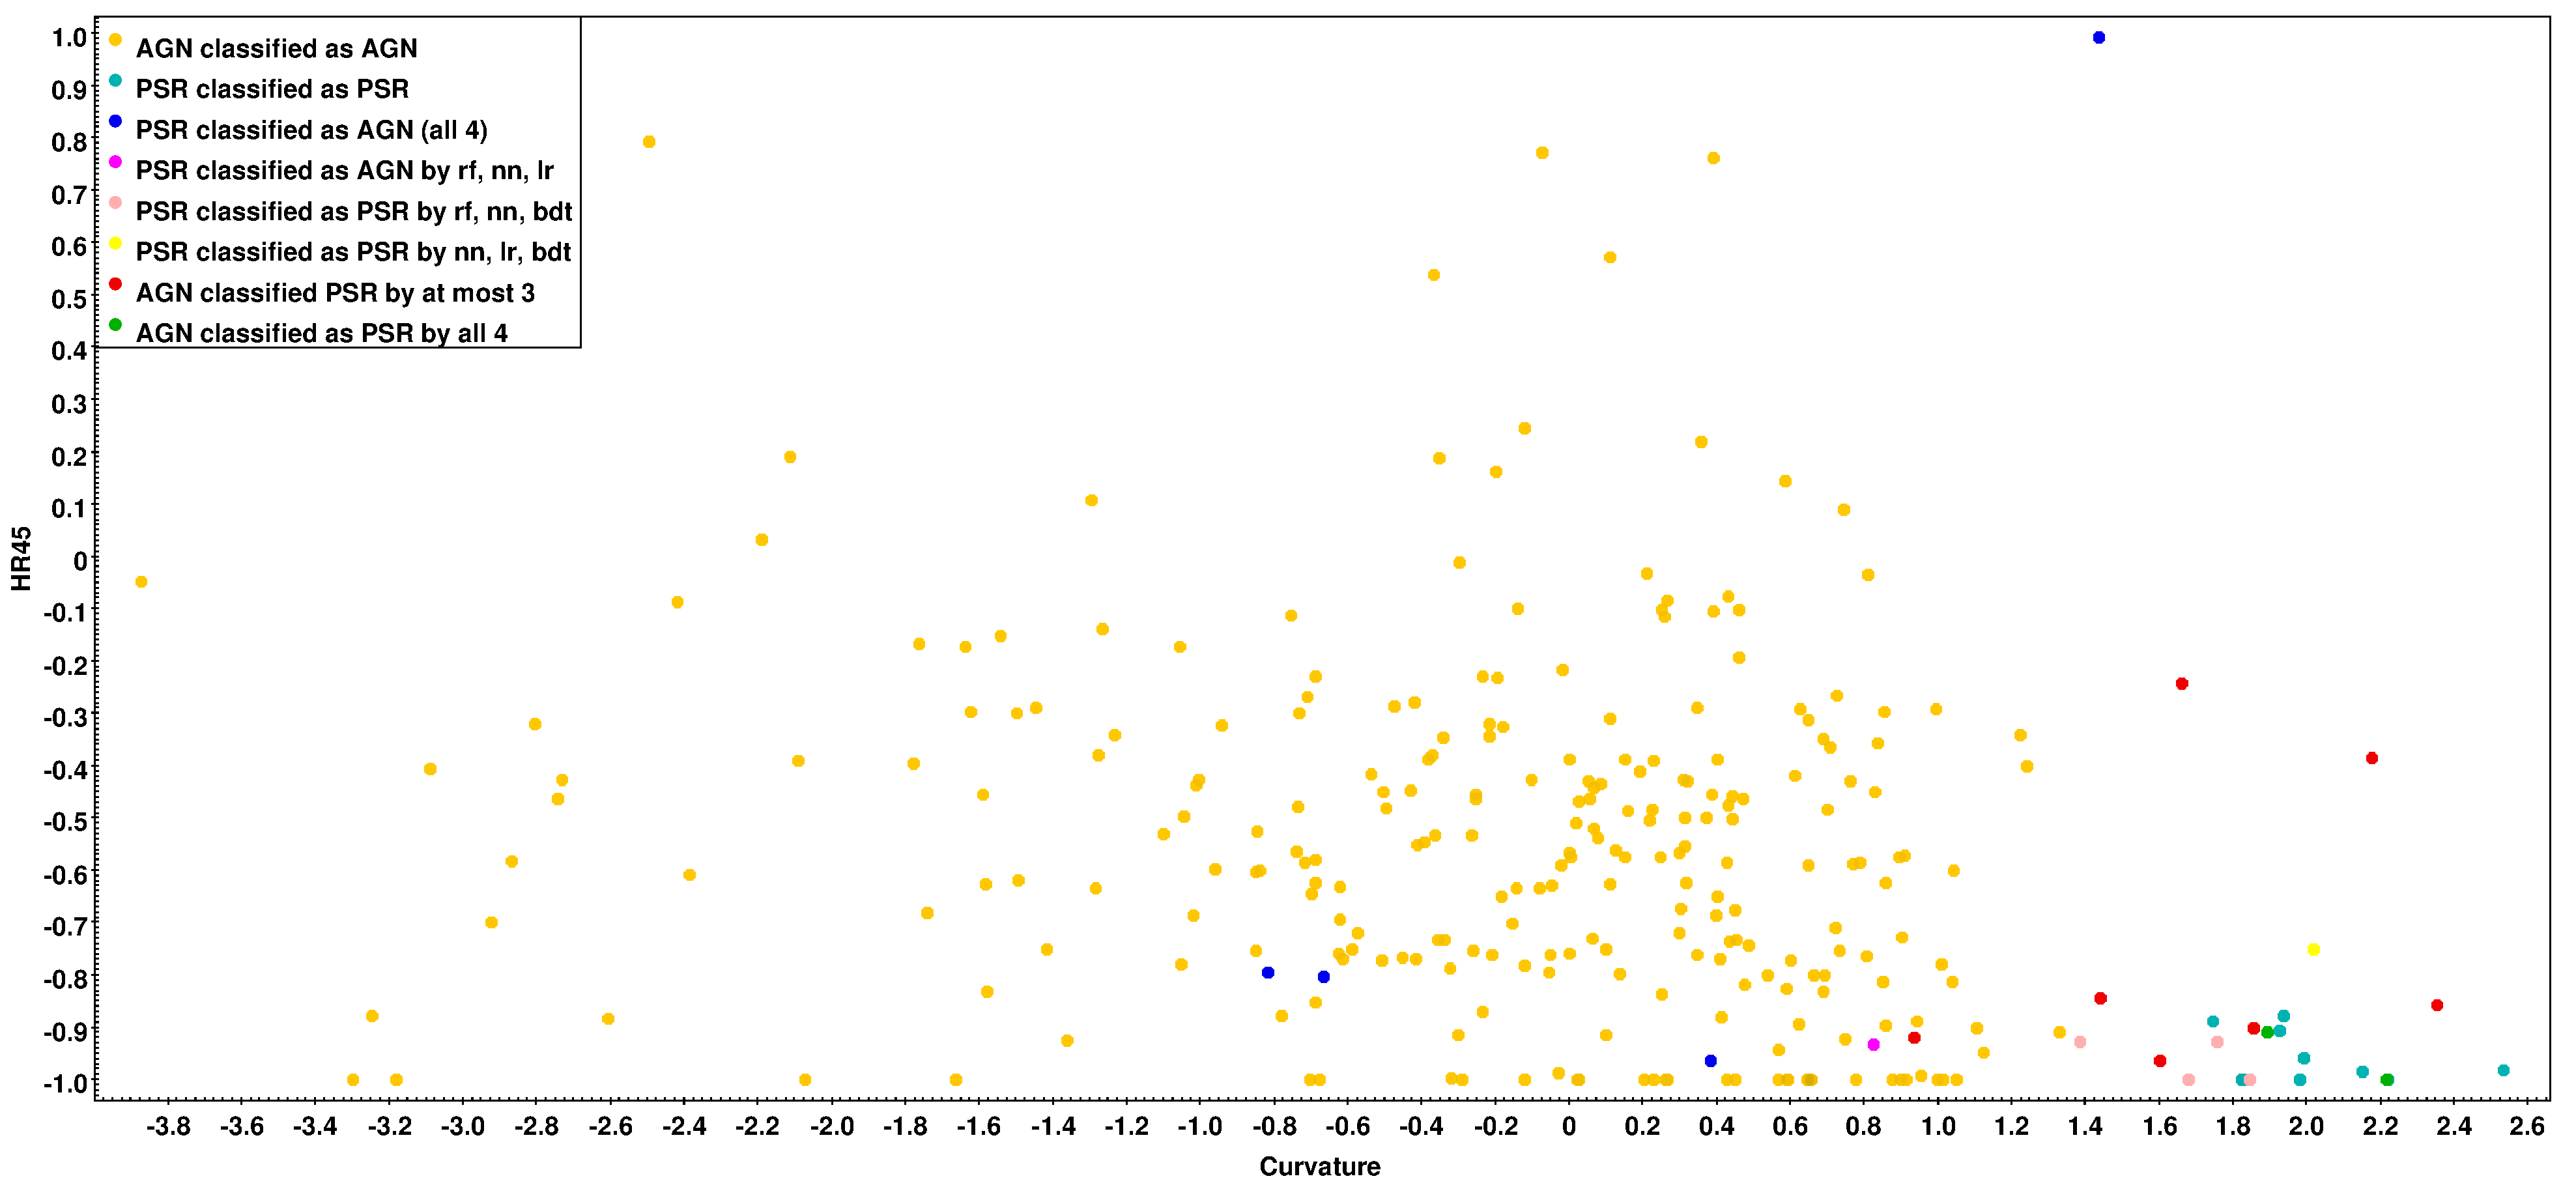
\includegraphics[width=\twopicsp\textwidth]{plots/final_catalog.pdf}
\label{fig:3FGL_vs_4FGL_classes}
\end{figure*}

As a result of the classification of 3FGL sources with the four ML algorithms,
we created probabilistic catalogs for unassociated and, separately, for associated 3FGL sources.
We have also subselected 278 unassociated 3FGL sources, which have PSR or AGN associations in 4FGL,
and saved them for convenience of comparison as a separate file, including characteristics from both 3FGL and 4FGL catalogs.
In the probabilistic catalogs we add columns with corresponding probabilities for each algorithm and each class,
i.e., provided that there are 4 algorithms and 2 classes, we add 8 columns.
Although the class probabilities for each algorithms should add up to one for every source, we still keep the columns for all classes for convenience.
Table \ref{tab:prob_cat} shows an example of the probabilistic catalog for a few unassociated 3FGL sources.
Notice that the first source is classified as a pulsar by BDT and as an AGN by RF, LR, and NN algorithms,
i.e., it has a label ``classified either as PSRs or AGNs'' in Figure \ref{fig:3FGL_vs_4FGL_classes}.
The second and third sources are classified as AGNs by all four algorithms, i.e., they will have a label
``classified only as AGNs'',
while the last source is classified as a pulsar by all four algorithms, i.e., it will have a label
``classified only as PSRs''.
Overall, there are 97 unassociated sources classified as pulsars by all four algorithms, 729 sources classified as AGNs by all four algorithms, and 182 sources with mixed classifications.
We summarize the results in Table \ref{tab:3FGL_prediction}, where we also show corrections for the presence of sources other than AGNs and pulsars.
Out of 97 sources classified as pulsars, 6 sources have counterparts in Parkes survey \cite{Camilo2015} within 2 arc minutes (see Table \ref{tab:parkes}).




\pgfplotstableread[col sep=comma]{data/catalogs/3FGL_unassoc_vs_4FGL_assoc.csv}\loadedtable
\begin{table}
\pgfplotstabletypeset[columns={Source_Name_3FGL,AGN_BDT,AGN_RF,AGN_LR,AGN_NN},
column type=l,
string type,
every head row/.style={before row={\toprule & \multicolumn{4}{c}{AGN Probability} \\},after row=\midrule,},
every last row/.style={after row=\vdots },
columns/Source_Name_3FGL/.style={column name=Source\_Name},
columns/AGN_BDT/.style={column name=BDT,numeric type,fixed,precision=3},
columns/AGN_NN/.style={column name=NN,numeric type,fixed,precision=3},
columns/AGN_RF/.style={column name=RF,numeric type,fixed,precision=3},
columns/AGN_LR/.style={column name=LR,numeric type,fixed,precision=3},
skip rows between index={4}{242}
]\loadedtable
\caption{\label{tab:prob_cat}
Example of the AGN classification probabilities for a few unassociated sources in the 3FGL catalog.}
\end{table}

\begin{table}[!h]
\resizebox{0.45\textwidth}{!}{
    \tiny
 %  \centering
    \renewcommand{\tabcolsep}{0.3mm}
\renewcommand{\arraystretch}{1.5}

    \begin{tabular}{| l |c|c|c|}
    \hline
    Correction for other sources & AGNs & Pulsars & Mixed \\
    \hline
    Uncorrected &  729 & 97  &  182 \\
    \hline
    Corrected & 708.0  & 81.5  & 164.5 \\
    \hline
     
    \end{tabular}}
    \vspace{0.2cm}
    \caption{Expected number of AGNs and pulsars among the unassociated 3FGL sources.
    Uncorrected (corrected) rows show the number of predicted AGNs and pulsars among the unassociated sources, which are
    uncorrected (corrected) for the presence of sources other than AGNs and pulsars among the unassociated sources.}
    \label{tab:3FGL_prediction}
\end{table}



\pgfplotstableread[col sep=comma]{data/catalogs/3fgl_unassoc_predictions_matches_with_Parkes(2015)_1.csv}\loadedtable
\begin{table}
\pgfplotstabletypeset[columns={3FGL,GLON,GLAT,Separation},
every head row/.style={before row={\toprule},after row=\midrule,},
every last row/.style={after row=\midrule },
columns/3FGL/.style={column name=Source\_Name,string type},
columns/GLON/.style={column name=GLON,numeric type,fixed,precision=1},
columns/GLAT/.style={column name=GLAT,numeric type,fixed,precision=1},
columns/Separation/.style={column name=Sep (arksec),numeric type,fixed,precision=1}
]\loadedtable
\caption{\label{tab:parkes}
Connection of unassociated 3FGL sources classified as PSRs with Parkes PSRs.}
\end{table}



\subsection{Prediction for unassociated source in the 4FGL catalog}
\lb{sec:4FGLprediction}

Building upon what we had done so far we were now ready to construct a probabilistic classification of sources in the 4FGL catalog.
As in the previous section, we use for training and testing sources associated with either AGNs or pulsars and have no missing values.
We then calculate the classification probabilities of AGN and PSR classes for both the associated and the unassociated sources.
The 4FGL catalog has higher number of features, especially due to the difference in modeling of the spectra compared with the 3FGL catalog. 
We selected 31 of these features and looked for the correlation among them. If any feature was correlated or anti-correlated with a Pearson index of $\pm$0.75 or higher with another feature, then only one of these features was kept. 
%The correlation matrix is shown in Figure \ref{fig:corr_mat}.
The resulting 16 features are:
GLON, GLAT, ln(Pivot\_Energy), ln(Flux1000), PL\_Index, Unc\_LP\_Index, LP\_beta, LP\_SigCurv, Unc\_PLEC\_Expfactor, PLEC\_Exp\_Index, hr12, hr23, hr34, hr45, hr56, hr67, ln(Variability\_Index).
Some of these features are directly related to the features, which we used in the 3FGL catalog,
e.g., GLAT, PL\_Index (instead of Spectral\_Index), LP\_SigCurv (instead of ln(Signif\_Curve)), ln(Variability\_Index), hardness ratios (in the 4FGL catalog there are two more energy bins compared to the 3FGL catalog).

\begin{comment}
\begin{figure*}[h]
\centering
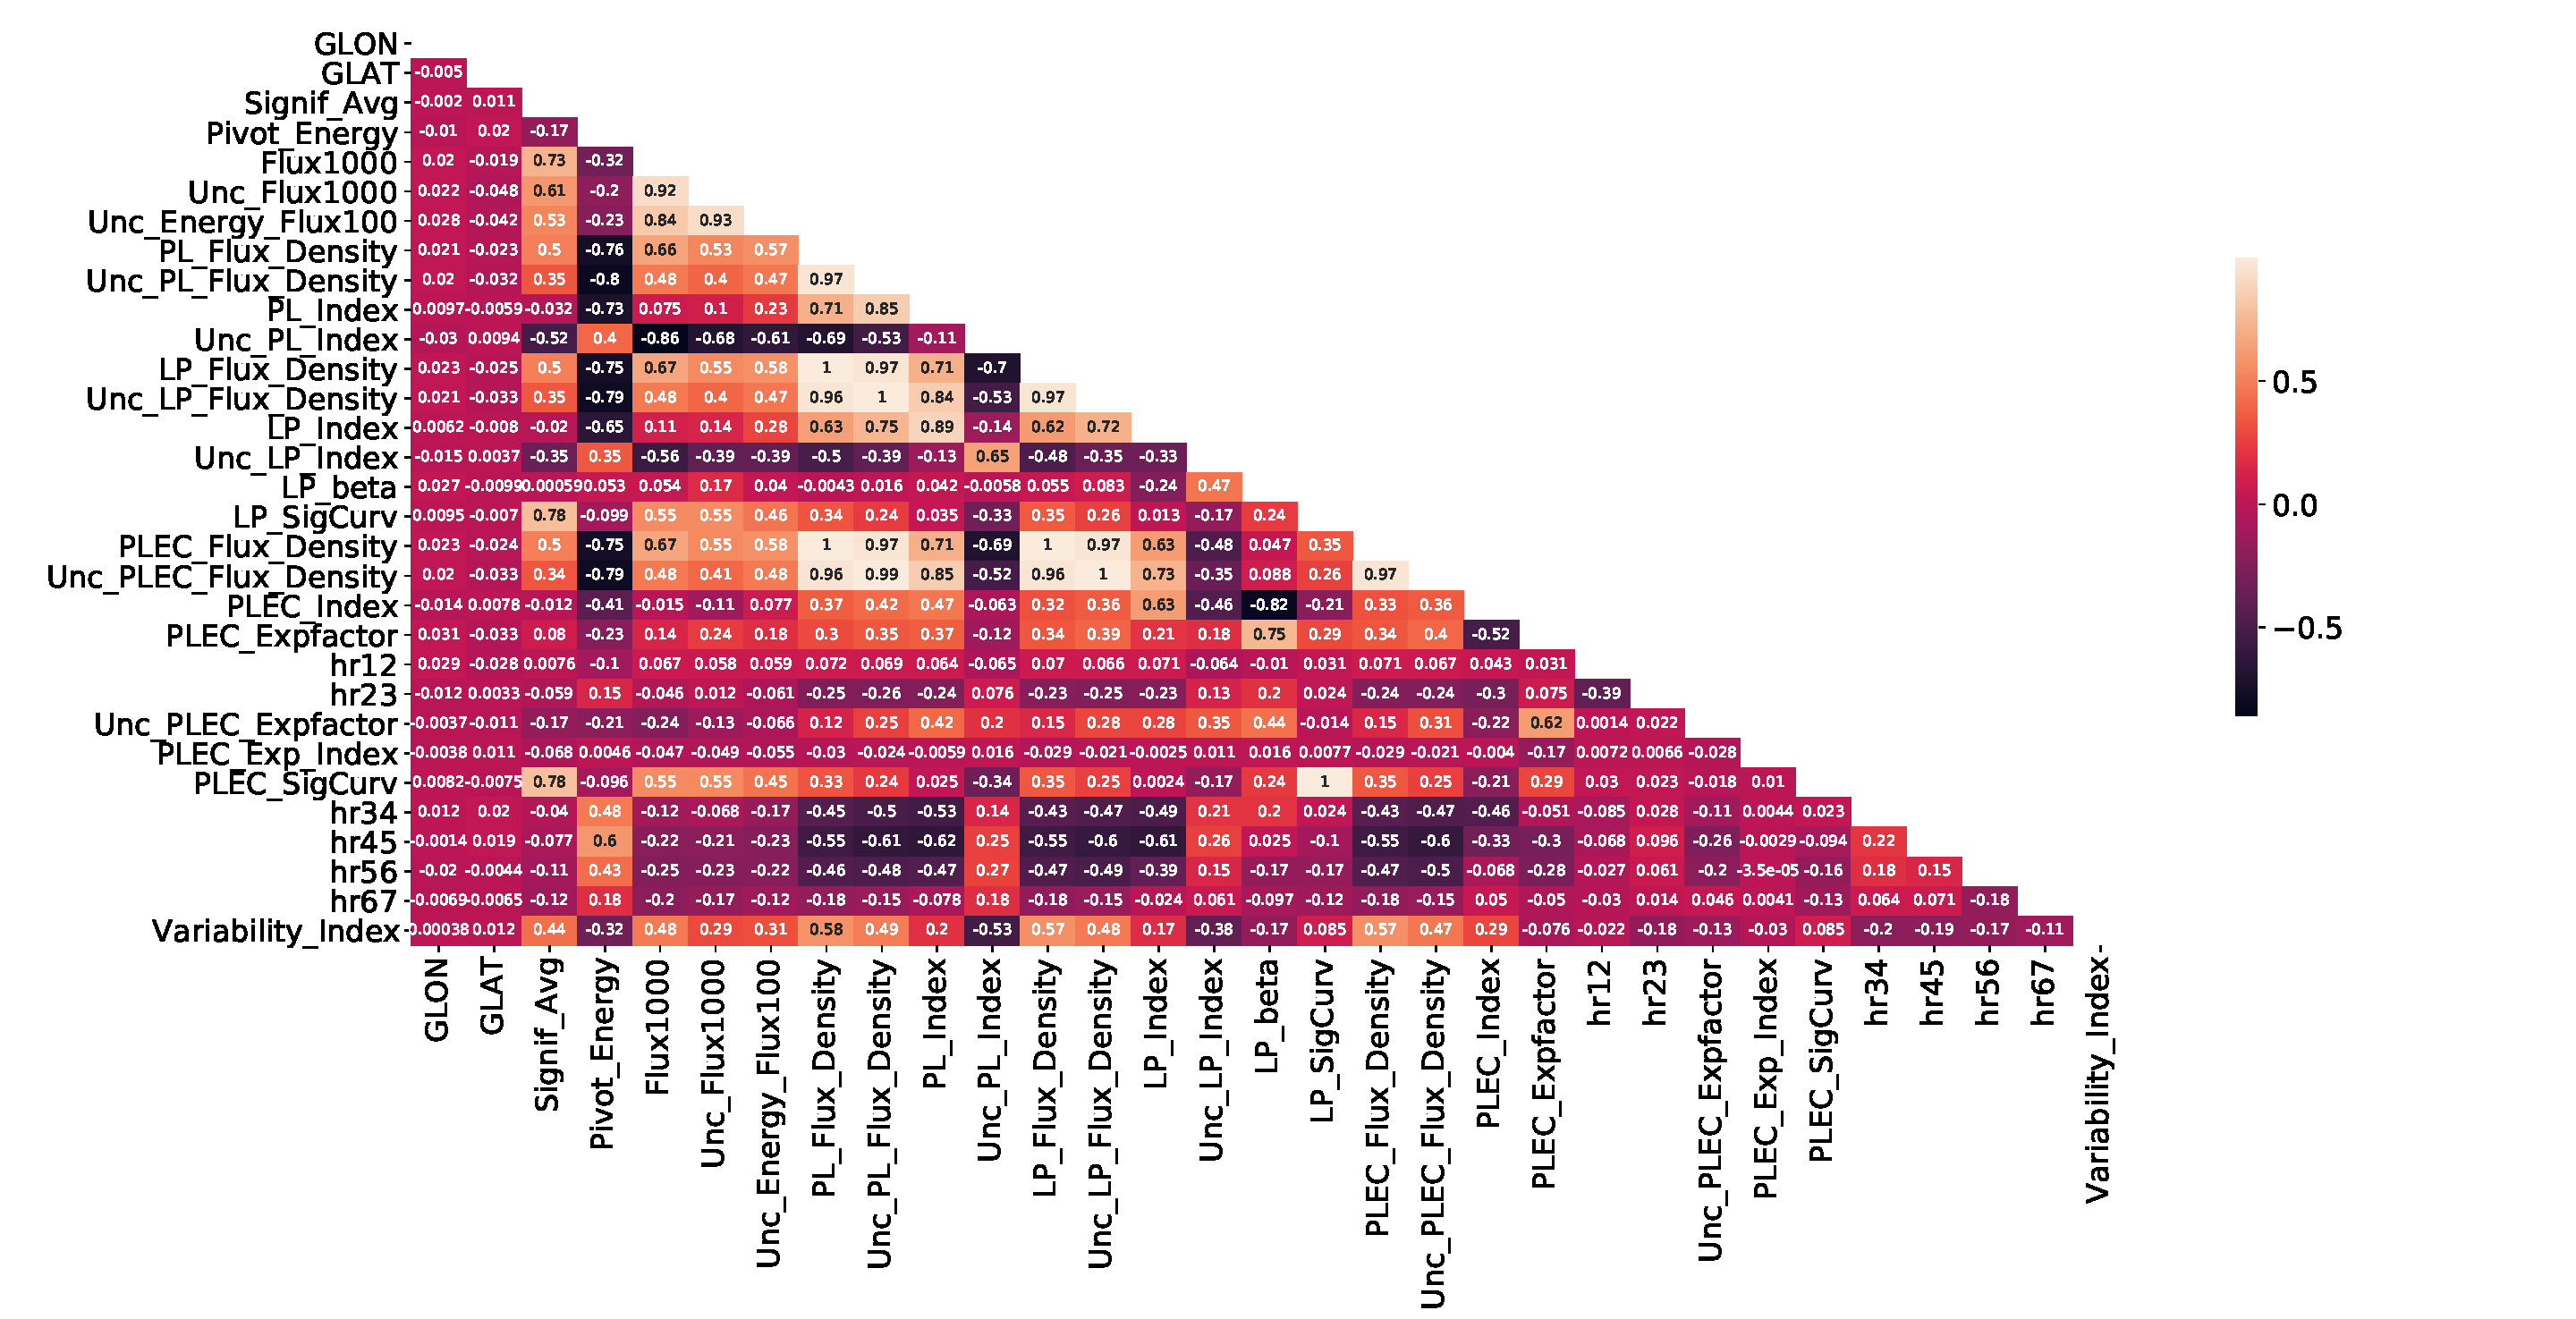
\includegraphics[width=\textwidth]{plots/correlation_4fgl_assoc.pdf}
%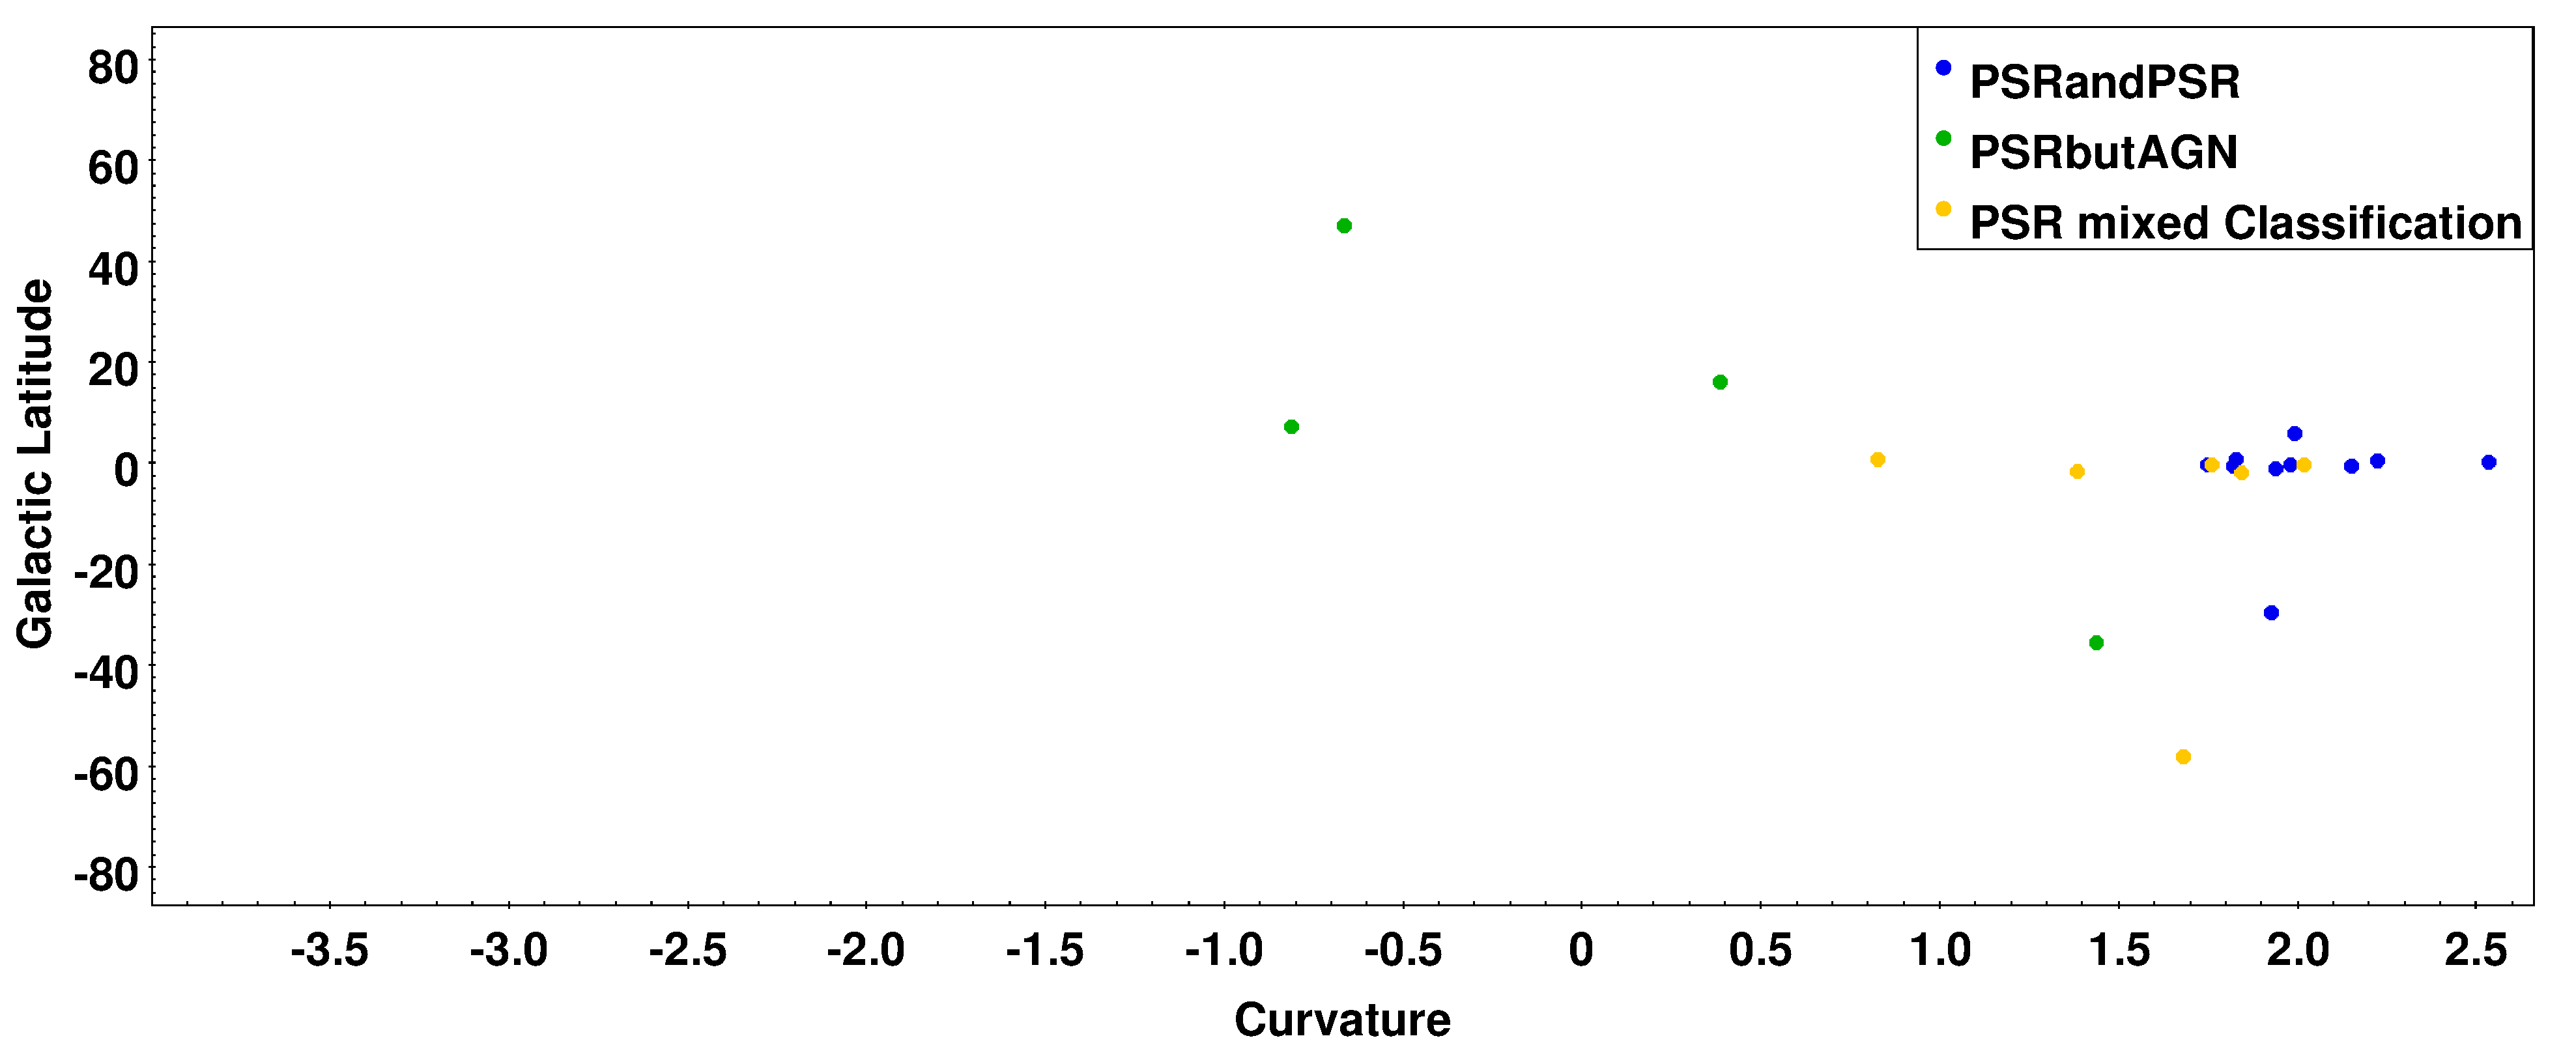
\includegraphics[width=\twopicsp\textwidth]{plots/PSR3.pdf}
\caption{Corelation matrix for 4FGL associated data }
%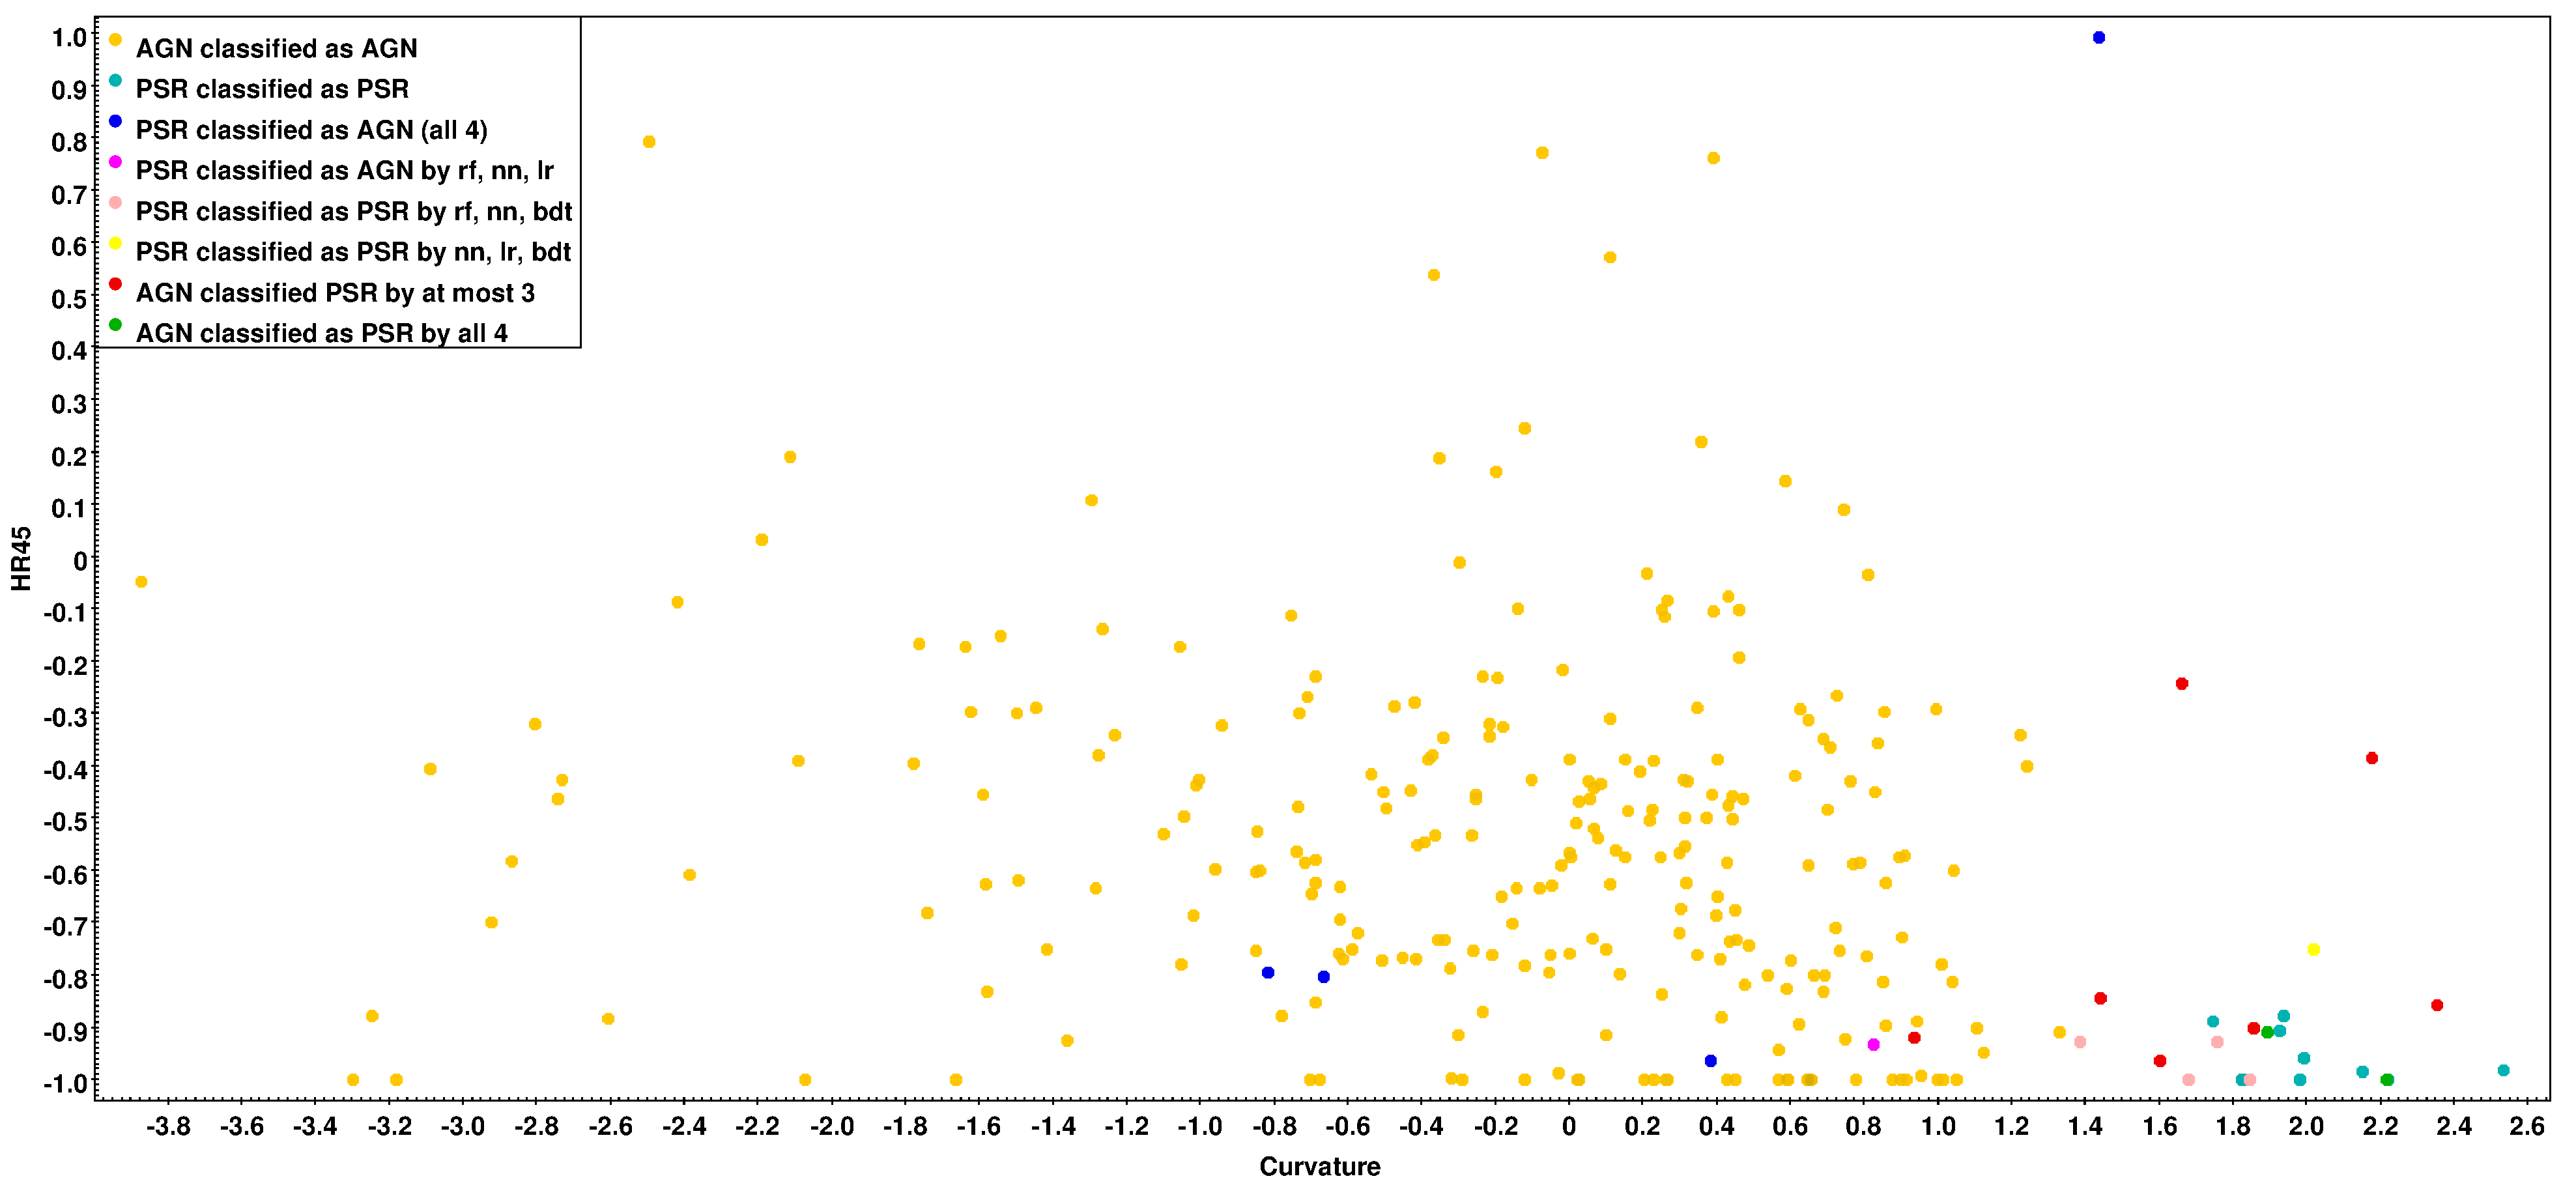
\includegraphics[width=\twopicsp\textwidth]{plots/final_catalog.pdf}
\label{fig:corr_mat}
\end{figure*}
\end{comment}

For this part, we do not perform another preliminary analysis of the algorithms, i.e., we used the same hyperparameters for the four algorithms as in the construction of the probabilistic catalog based on the 3FGL catalog, except for the neural network where we increased the number of neurons to 16.
We retrain these algorithms using the 16 features for the 4FGL sources.
The corresponding accuracies are reported in Table \ref{tab:selected_algs2}.
All algorithms have a better accuracy for the 4FGL catalog compared to the 3FGL catalog, which is likely due to a higher number of features and more associated sources used as training data. 

% (same as the number of features). However, due to the number of features being higher, we hypothesized that the Neural Network should under-perform as compared to before.

\begin{table}[!h]
\resizebox{0.45\textwidth}{!}{
    \tiny
 %  \centering
    \renewcommand{\tabcolsep}{0.3mm}
\renewcommand{\arraystretch}{1.5}

    \begin{tabular}{|c|c|c|}
    \hline
    Algorithm&Parameters & Testing Accuracy \\
    \hline
    RF& 50 trees, max depth 6  &98.27\\
    \hline
    NN & 300, 16 Neurons, Adam & 98.08\\
    \hline %\midrule   -> aakash do you mean this?
    BDT & 100 trees, max depth 2    &   98.23\\
%    \hline %\midrule   -> aakash do you mean this?
%    BDT & 200 trees, max depth 2    &   95.8  \\
    \hline
    LR & LBFGS solver, 200 iterations & 98.08\\
    \hline
     
    \end{tabular}}
    \vspace{0.2cm}
    \caption{Accuracy of the 4 selected algorithms on 4FG associated data.}
    \label{tab:selected_algs2}
\end{table}

The expected number of AGNs and pulsars among the unassociated source in the 4FGL catalog is reported in Table \ref{tab:4FGL_prediction}.
The ``AGNs'' column shows the number of unassociated sources where all four algorithms from table \ref{tab:selected_algs2} give the probability for a source to be an AGN above 50\%.
Similarly the ``Pulsars'' column shows the number of unassociated sources where all four algorithms predict the source to be more likely a pulsar.
The ``Mixed'' column shows the number of sources with mixed classification, i.e., some algorithms predict that the source is more likely an AGN while the other algorithms predict that it is more likely a pulsar.
In the ``Uncorrected'' row we do not take into account that there can be sources other than AGNs or pulsars among the unassociated sources.
We correct for the presence of the other sources by assuming that the fraction of AGN-like and pulsar-like sources among the other sources is the same for associated and for unassociated sources.
In particular, we denote by $N_{\rm AGN}$ the number of unassociated sources with AGN-like classification by all four algorithms,
by $N_{\rm AGN}^{\rm ass\,other}$ the number of sources with AGN-like classification among associated other sources,
by $N_{\rm ass}$ ($N_{\rm unass}$) the total number of associated (unassociated) sources.
The number of AGN-like sources among the unassociated source corrected for the presence of other sources is estimated as

\be
\lb{eq:other_correction}
N_{\rm AGN}^{\rm corr} = N_{\rm AGN} - N_{\rm AGN}^{\rm ass\,other} \,\frac{N_{\rm unass}}{N_{\rm ass}}.
\ee
Analogous corrections are applied for the number of unassociated sources with pulsar-like classification by all four algorithms,
and for unassociated sources with mixed classification.

\begin{table}[!h]
\resizebox{0.45\textwidth}{!}{
    \tiny
 %  \centering
    \renewcommand{\tabcolsep}{0.3mm}
\renewcommand{\arraystretch}{1.5}

    \begin{tabular}{| l |c|c|c|}
    \hline
    Correction for other sources & AGNs & Pulsars & Mixed \\
    \hline
    Uncorrected &  949 & 137  &  250 \\
    \hline
    Corrected & 896.3  & 115.5  & 221.3 \\
    \hline
     
    \end{tabular}}
    \vspace{0.2cm}
    \caption{For definitions see Table \ref{tab:4FGL_prediction}.}
    \label{tab:4FGL_prediction}
\end{table}

Finally, we looked at sources which were unassociated in both 3FGL and 4FGL (306 sources). 38 sources are predicted to be PSRs using 3FGL features and 71 sources using 4FGL features. This leads to a total of 29 sources which were predicted by all four algorithms to be PSRs for features taken from both 3FGL and 4FGL. Amongst these 29 PSRs, four are again belonging to the Parkes survey (of the other two, one is now associated as a PSR in 4FGL, and the second is not there in 4FGL). These 29 sources can be looked at as having the strongest case to be PSRs amongst all unassociated sources. 

